\section{Pre-training Dataset}\label{sec:method}


To improve VLA models for strong generalization and practicality across diverse embodiments and dynamic environments, we redesign the data processing pipeline and curate a large-scale pretraining dataset of approximately 60,000 hours, as illustrated in~\cref{fig:data_demo}. The redesigned data processing pipeline is shown in~\cref{fig:data_process}.

\begin{figure}[t]
\centering
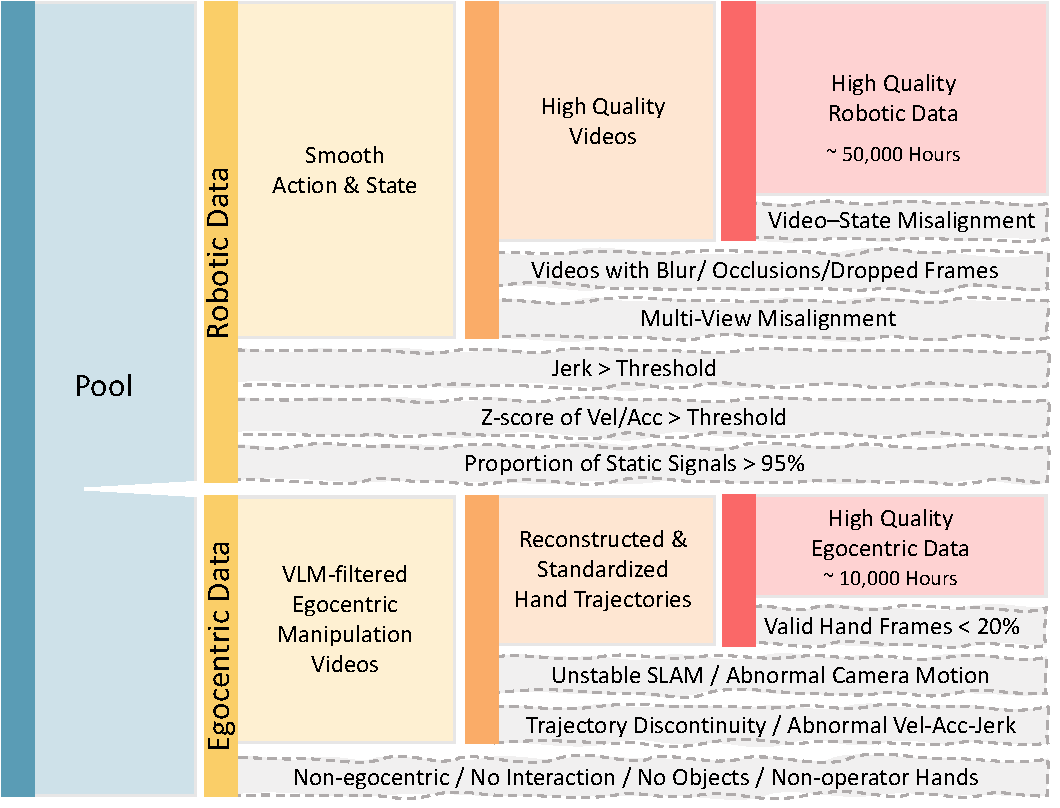
\includegraphics[width=0.7\linewidth]{figures/data_process.pdf}
\caption{Data processing pipeline.}
\label{fig:data_process}
\end{figure}

\subsection{Data Curation and Pre-Processing}

\subsubsection{Robotic Data}


We collect approximately 90,000 hours of data from 20 embodiments, spanning single-arm, dual-arm, and mobile robotic platforms equipped with dexterous hands or grippers. Based on the collected data, we employ a redesigned data processing pipeline to filter noisy samples, yielding 50,000 hours of high-quality robotic data.


We first compute the third-order finite difference (jerk) of the action and state signals, along with the Z-scores of their first-order derivatives (velocity) and second-order derivatives (acceleration), to assess trajectory smoothness. An episode is discarded if either the jerk or any derivative Z-score exceeds a predefined threshold. 
These thresholds are set separately for each embodiment.
Moreover, we measure the duration within an episode during which all state and action signals exhibit only small variations or remain unchanged. If this duration accounts for more than 95\% of the entire episode, the episode is also discarded.



To verify consistency between the videos and state signals, we project the robot onto the image plane using the corresponding URDF and replay the recorded states. 
Human annotators are employed to identify discrepancies between the projected robot and the videos to ensure that the state signals and videos are correctly recorded, and samples with such misalignment are removed. Meanwhile, videos with blur, severe occlusions, dropped frames, or misalignment across multiple views are filtered out by human annotators during the annotation process.


\begin{table}[t]
\centering
\caption{Statistical overview of robot manipulation data in LingBot-VLA-2.0.}
\label{tab:linbotvla_robot_data}
\small
\setlength{\tabcolsep}{5pt}
\begin{tabular}{lcccccc}
\toprule
Robot Type & EE type &Hand/Gripper DoF & Arm DoF & Body DoF$^{*}$ & Total DoF & Policy Frequency\\
\midrule
\multicolumn{5}{l}{\textbf{Single-Arm Robots}} \\
Franka & Grppier&1&7&0&8&30 \\
Flexiv Rizon 4 & Grppier  &1&7&0&8&30  \\
\midrule
\multicolumn{5}{l}{\textbf{Dual-Arm Robots}} \\
AgileX & Grppier &2&12&0&14&30\\
ARX Lift2& Grppier &2&12&0&14&30\\
UR7e & Grppier  &2&12&0&14&30  \\
\midrule
\multicolumn{5}{l}{\textbf{Half-Humanoid}} \\
AgiBot G1 & Grppier      &2&14&4&20&30 \\
Galbot G1 & Grppier& 2 & 14 & 6& 22 & 30 \\
Moz1 & Grppier  &2&14&0&16&30  \\ 
Realman Rs-02 & Grppier & 2 & 14 & 1 & 17 & 30 \\
Galaxea R1Pro & Grppier & 2 & 14 & 7 & 23 & 15 \\
Galaxea R1Lite & Grppier & 2 & 12 & 3 & 17 & 15 \\
Astribot S1 & Grppier & 2 & 14 & 9 & 25 & 30 \\
Zerith H1 & Grppier & 2 & 14 & 7 & 23 & 30 \\
\midrule
\multicolumn{5}{l}{\textbf{Humanoid}} \\
Leju KUAVO 4 Pro & Grppier/Hand&2/12&14&5&21/31&30 \\
Tienkung & Grppier& 2& 14 & 0 & 16 & 30\\ 
QingLong & Grppier& 2& 14 & 0 & 16 & 30\\ 
MagicBot Gen1&Grppier& 2& 14 & 4 & 20 & 30 \\
Unitree G1 & Hand& 12 & 14 & 0 & 26 & 30  \\
Fourier GR-2 &Hand & 12 & 14 & 6 & 32 &30\\
AgiBot A2 &Hand & 12 & 14 & 2 & 28 & 30 \\
\midrule
\multicolumn{5}{l}{\textbf{Humanoid}} \\
Ego & - &- &14 &- &14  &30\textasciitilde 60 \\
\midrule
\multicolumn{6}{l}{\textbf{Total: 20 embodiments}} & \textbf{60000h} \\
\bottomrule
\end{tabular}
\begin{tablenotes}
\footnotesize
\item[] $*$ The total number of body DoF used for model training.
\end{tablenotes}
\end{table}

\subsubsection{Egocentric Data}

We construct an egocentric human video pool of approximately 20,000 hours and retain around 10,000 hours of high-quality training data after filtering, reconstruction, standardization, and quality control. 
We first apply a unified video-level VLM pre-filter to all candidate videos, regardless of source. This step removes videos that do not satisfy the egocentric manipulation assumption, such as third-person observation videos, scene-walking videos, videos without clear hand-object interaction, or videos without manipulable objects. We also filter out videos where non-operator hands appear prominently, since such clips can break the association between the camera wearer's observation and the corresponding hand motion. Applying this VLM filtering stage before downstream processing reduces unnecessary annotation and reconstruction cost, especially for action-free videos that would otherwise require SLAM and hand pose estimation.

After VLM pre-filtering, we process the remaining data according to whether action or hand trajectory labels are available. For data with existing action or hand trajectory labels, including action-labeled open-source datasets and in-house data, we perform metadata organization, timestamp alignment, coordinate transformation, and trajectory completeness checking, converting all samples into a standardized hand trajectory format. For action-free egocentric human videos, we run egocentric SLAM to estimate camera intrinsics and per-frame camera extrinsics, and then apply hand pose estimation to recover MANO parameters in the camera coordinate frame. By combining the estimated hand poses with camera poses, we lift the hand motion into the world coordinate frame and obtain temporally continuous hand trajectories.

We then apply trajectory-level quality control to the reconstructed and standardized data. We filter out videos with insufficient valid hand pose coverage, using a 20\% valid-frame ratio as the minimum threshold. We also remove clips with unstable SLAM trajectories, identified by abnormal second-order changes in the estimated camera motion, such as sudden translational or rotational acceleration. In addition, we reject hand trajectories with sudden discontinuities, abnormal displacement, velocity, acceleration, or jerk, as well as samples that violate human physiological constraints, such as unreasonable hand positions, inter-hand distances, motion ranges, or poses.

Finally, all valid samples are stored as hand trajectories in the world coordinate frame. During training, when a frame is sampled as the current observation, we transform the future hand trajectory from the world coordinate frame into the current camera coordinate frame using the camera extrinsic of that frame:
\begin{equation}
    \mathbf{p}_{\tau}^{C_t} = \mathbf{T}_{C_t \leftarrow W} \mathbf{p}_{\tau}^{W}.
\end{equation}
Here, $\mathbf{p}_{\tau}^{W}$ denotes the hand trajectory in the world coordinate frame, and $\mathbf{T}_{C_t \leftarrow W}$ denotes the transformation from the world coordinate frame to the camera coordinate frame of the sampled frame $t$. With this design, the world coordinate frame serves as the unified trajectory storage space, while the current camera coordinate frame serves as the training-time action representation. This unifies trajectory formats across open-source and in-house egocentric human videos, and decouples hand motion from egocentric camera motion during training.

\subsubsection{Unified Action Representation} 

To jointly learn state and action representations from egocentric data and robotic data collected across multiple embodiments, we use a 55-dimensional canonical vector representation for both states and actions. This representation consists of 14 dimensions for arm joint position, 14 dimensions for end-effector pose, 2 dimensions for gripper position, 12 dimensions for hand joint position, 4 dimensions for waist position, 2 dimensions for head position, and 3 dimensions for mobility signal, as shown in~\cref{fig:data_dimension}. The remaining 4 dimensions are reserved.
The arm joint position and end-effector pose fields are defined to accommodate the maximum dimensionality of a dual-arm embodiment. Specifically, the end-effector pose of each arm is represented by XYZ coordinates and a rotation quaternion, resulting in 7 dimensions per arm. For single-arm data, only 6 or 7 dimensions are used for arm joint positions and 7 dimensions for the end-effector pose, while the remaining arm-related dimensions are padded.
Similarly, for robot embodiments that do not include specific body parts or have lower-dimensional signals, the corresponding dimensions are also padded.
The dimensional configurations for each embodiment are shown in~\cref{tab:linbotvla_robot_data}.

\begin{figure}[t]
\centering
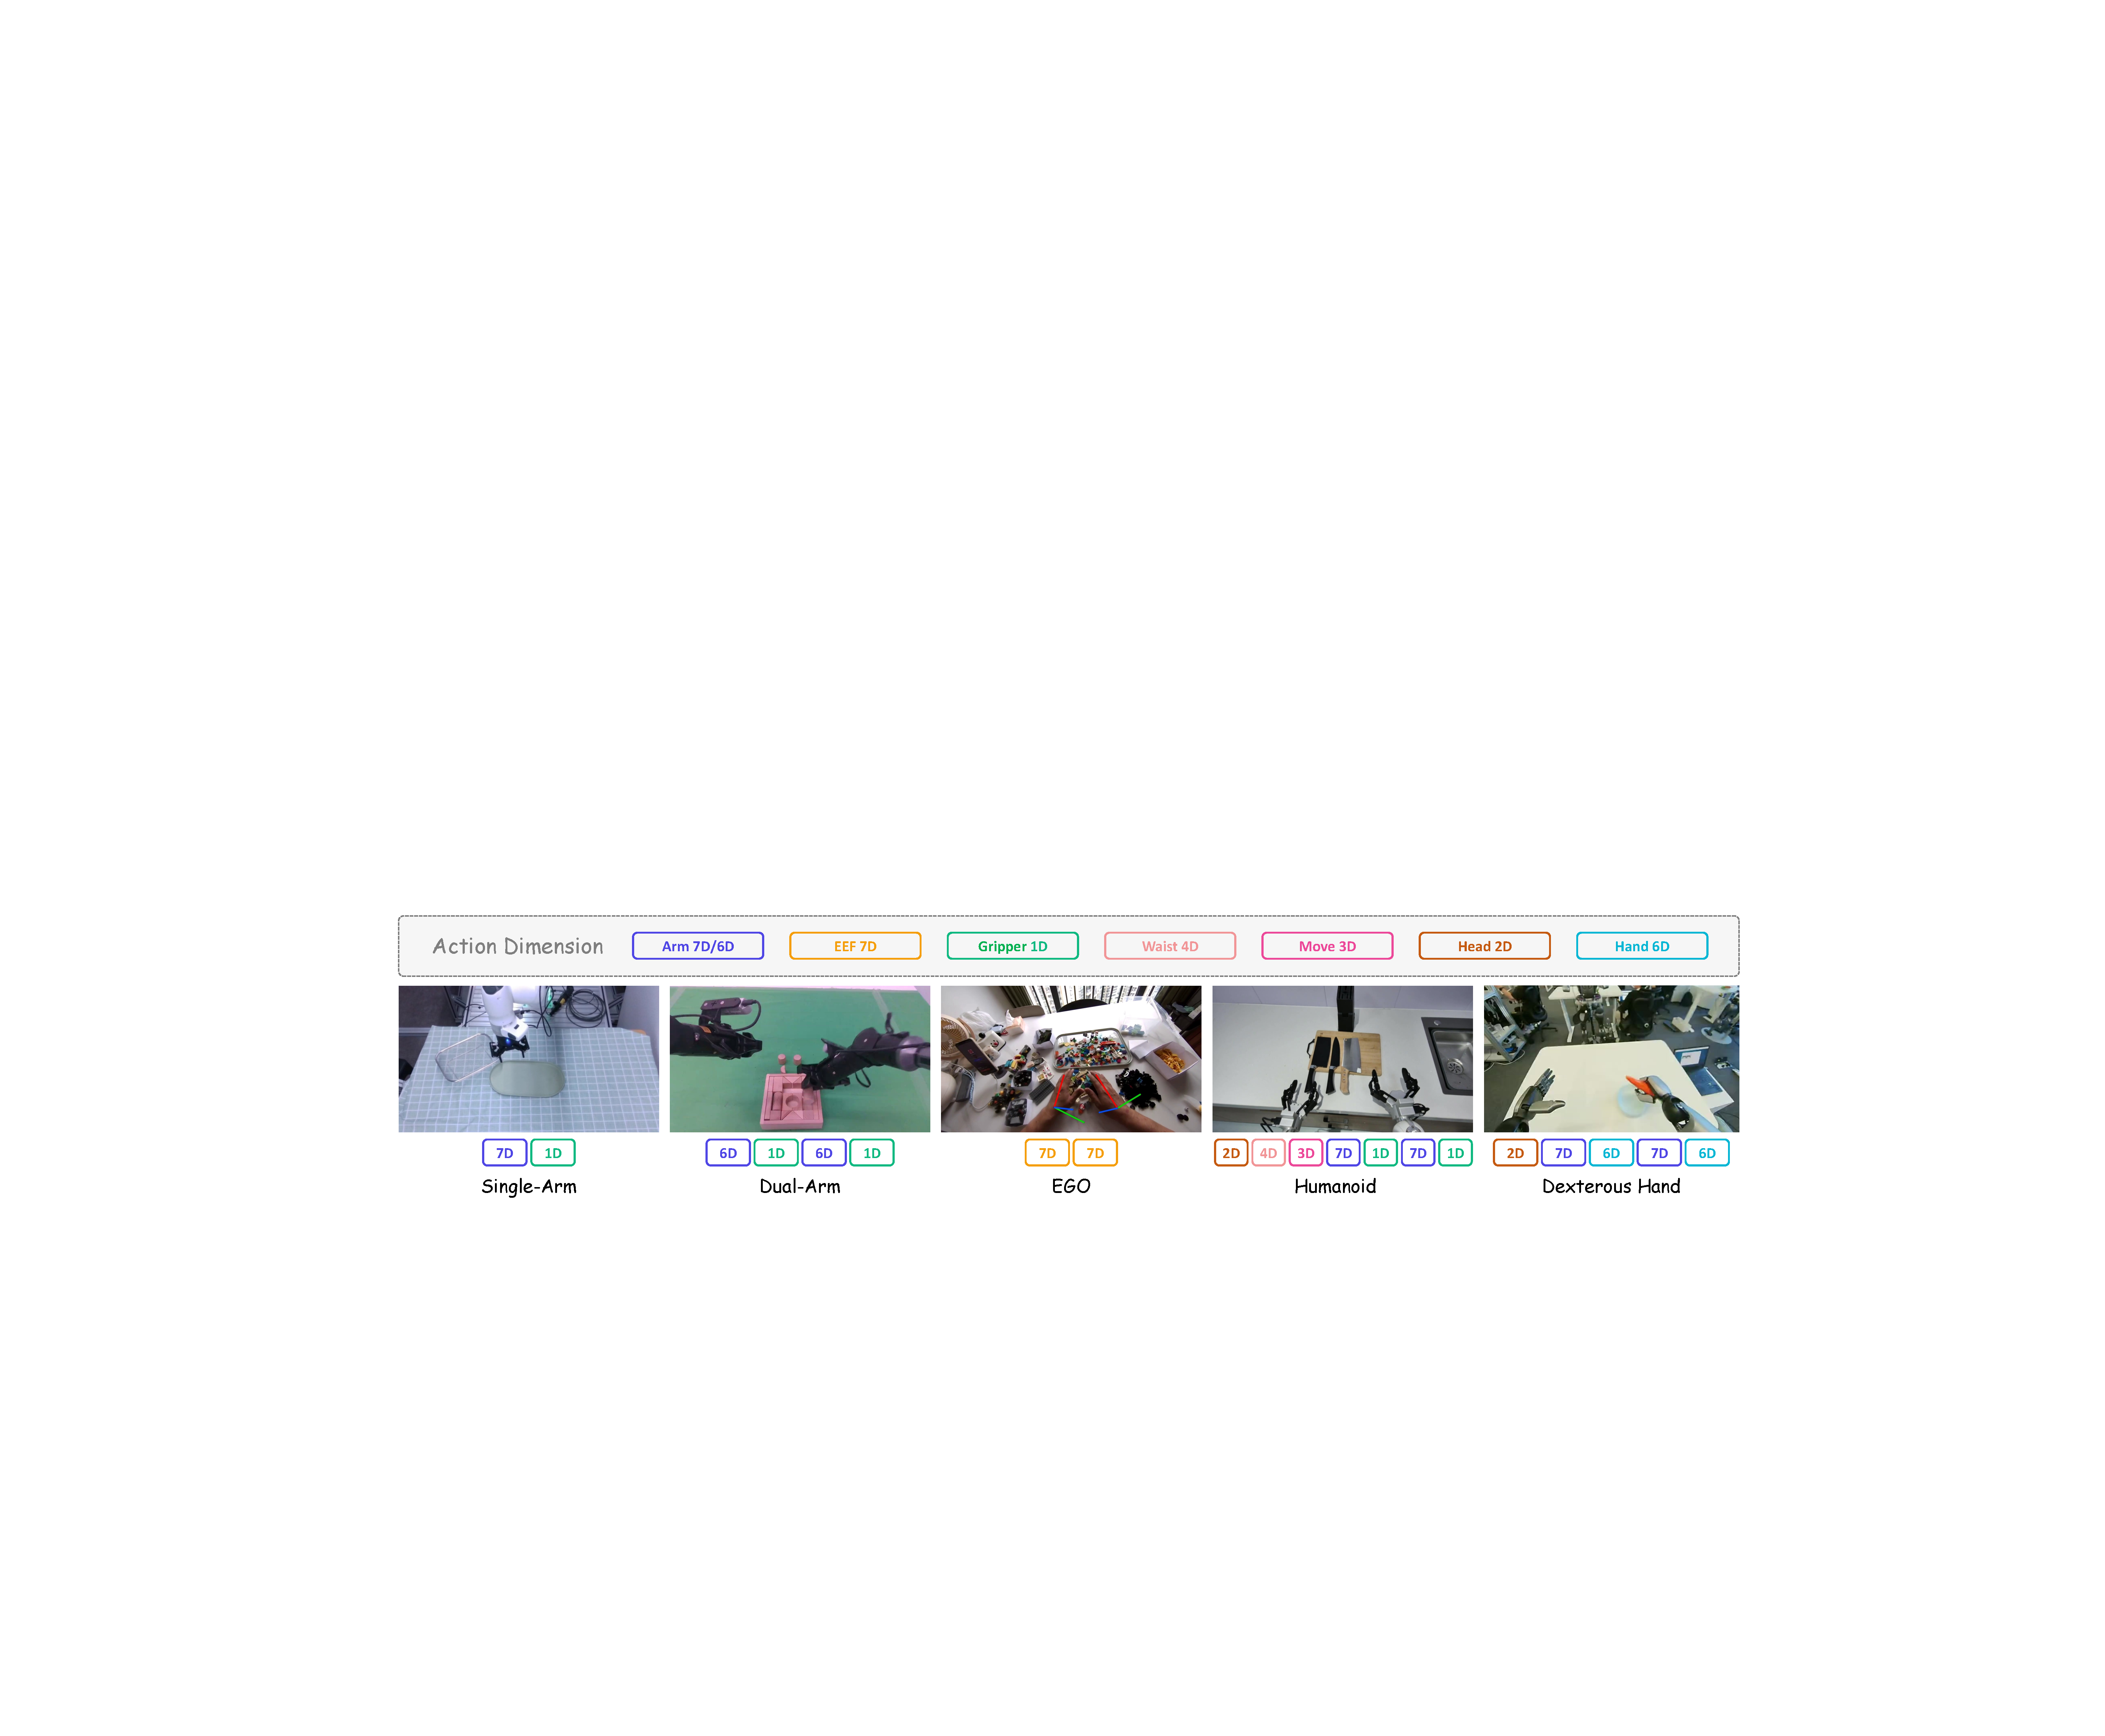
\includegraphics[width=\linewidth]{figures/data_dimension.pdf}
\caption{\textbf{Unified action representation}. We map heterogeneous embodiment controls into compact action vectors composed of shared body-part components.}
\label{fig:data_dimension}
\end{figure}

\subsection{Data Annotation}
\label{sec:data_annotation}

VLA pretraining benefits from manipulation videos paired with temporally aligned language supervision at both the task and subtask levels. We generate these annotations with a fully automated pipeline built on a vision--language model, and apply this pipeline across the pretraining dataset.

Specifically, we employ Qwen3.6-27B~\cite{qwen3.6-27b} to segment each manipulation video into a sequence of temporally contiguous subtasks and to generate the corresponding language instructions. For robotic platforms with multiple cameras, the overhead and wrist views are processed jointly to disambiguate gripper--object interactions. Each subtask is assigned an atomic action from a closed vocabulary of 18 categories (\cref{tab:subtask_vocab}), together with the primary object of interaction and a concise instruction. In addition, a single video-level instruction summarizes the overall task. The annotated objects form a diverse, open vocabulary, as visualized in~\cref{fig:object_cloud}.

To keep the segmentation granularity consistent, the model groups the grasp, carry, and release phases of a single interaction into one subtask, and introduces a temporal boundary only when the manipulated object changes, the action type changes, or a sustained pause marks a transition to a new sub-goal. As summarized in~\cref{fig:subtask_stats}, \emph{move} and \emph{transit} dominate in frequency, whereas fine-grained manipulations such as \emph{cut}, \emph{fold}, and \emph{stir} are rare but have considerably longer mean durations.


\begin{table}[t]
\centering
\small
\setlength{\tabcolsep}{5pt}
\renewcommand{\arraystretch}{1.08}
\caption{
Closed vocabulary for subtask annotation.
The vocabulary consists of 15 primitive manipulation actions and three auxiliary labels:
\texttt{transit} for empty-hand motion, \texttt{idle} for stationary arms, and
\texttt{other} for out-of-vocabulary actions.
}
\label{tab:subtask_vocab}
\begin{tabularx}{\columnwidth}{@{}>{\ttfamily}l X @{\quad} >{\ttfamily}l X@{}}
\toprule
\normalfont\textbf{Action} & \textbf{Description}
& \normalfont\textbf{Action} & \textbf{Description} \\
\midrule

\multicolumn{4}{@{}l}{\textbf{Primitive manipulation actions}} \\
\addlinespace[0.15em]
move   & Relocate an object
& fold   & Shrink flexible material \\
pour   & Tilt a container to dispense contents
& unfold & Expand flexible material \\
push   & Slide an unheld object
& wipe   & Move a tool across a surface \\
pull   & Draw an object closer
& stir   & Move a tool circularly in a container \\
rotate & Turn an object in place
& cut    & Sever a target with a blade \\
open   & Open a hinged or articulated object
& press  & Press a button, switch, or surface \\
close  & Close a hinged or articulated object
& attach & Insert or connect an object to a fitting \\
detach & Remove or disconnect an object from a fitting
&        & \\

\addlinespace[0.35em]
\midrule
\multicolumn{4}{@{}l}{\textbf{Auxiliary labels}} \\
\addlinespace[0.15em]
transit & Move the gripper without object interaction
& idle   & Keep the arms stationary \\
other   & Action outside the vocabulary
&        & \\

\bottomrule
\end{tabularx}
\end{table}


\begin{figure}[t]
\centering
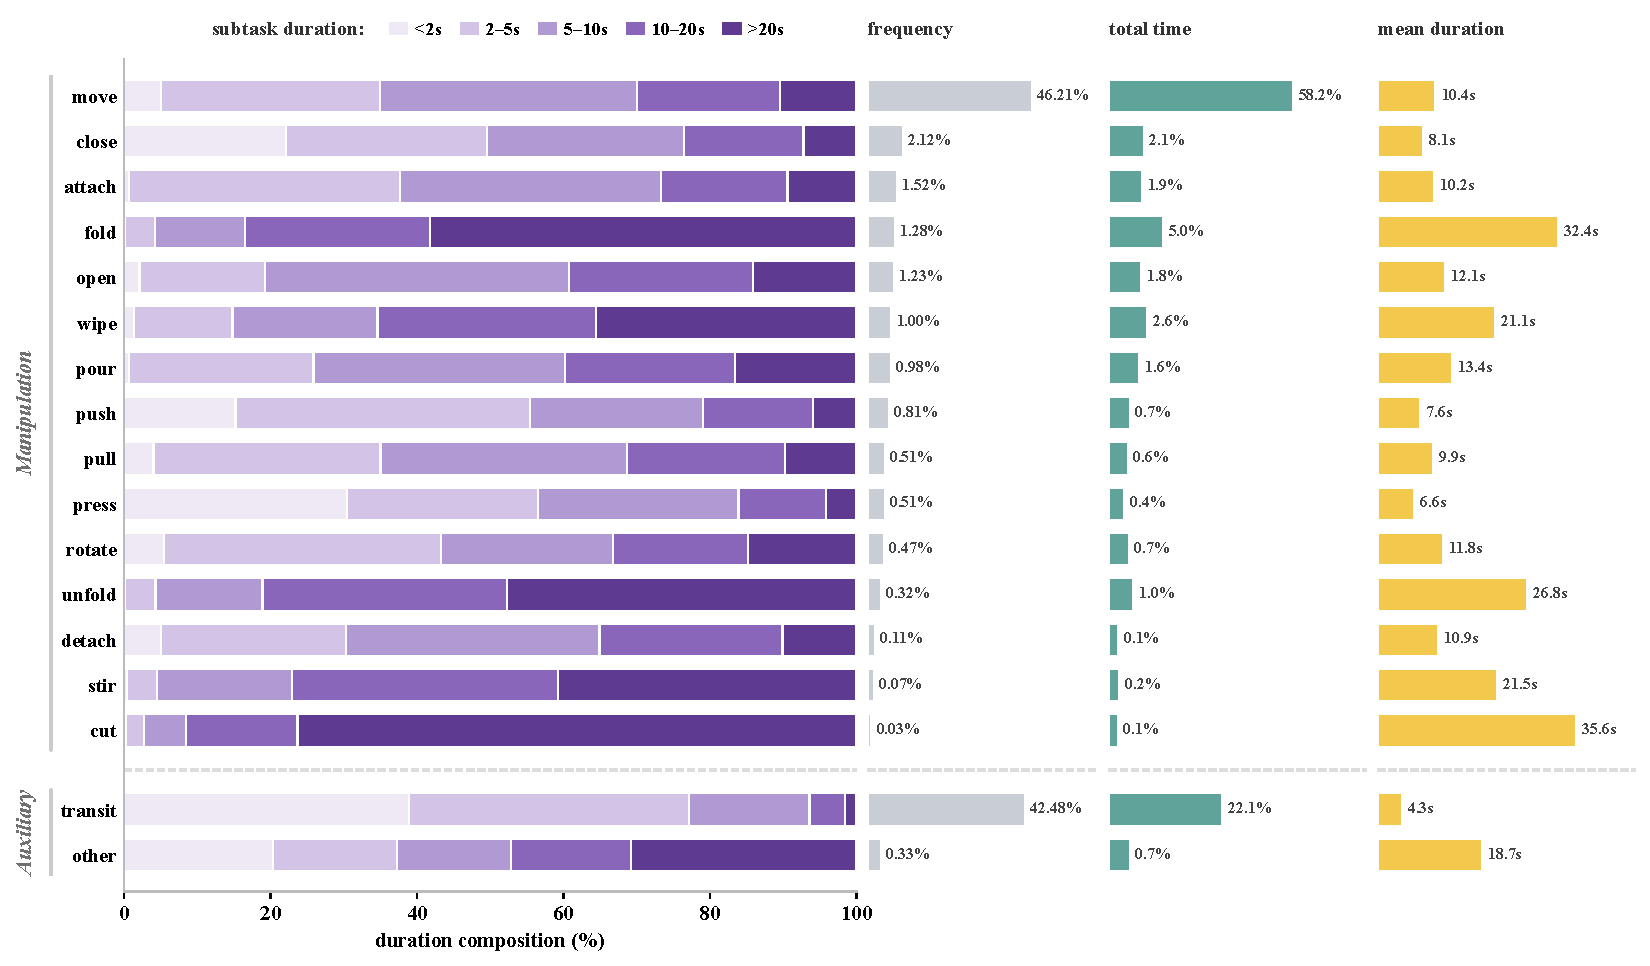
\includegraphics[width=\linewidth]{figures/Data_Annotation/subtask_duration_stats.pdf}
\caption{Per-action statistics of the subtask annotations: duration composition, \emph{frequency} (fraction of all subtasks), \emph{total time} (fraction of the total annotated time), and \emph{mean duration}. Actions are grouped as in~\cref{tab:subtask_vocab}; \emph{idle} is filtered out of the training data and omitted here.}
\label{fig:subtask_stats}
\end{figure}

\begin{figure}[t]
\centering
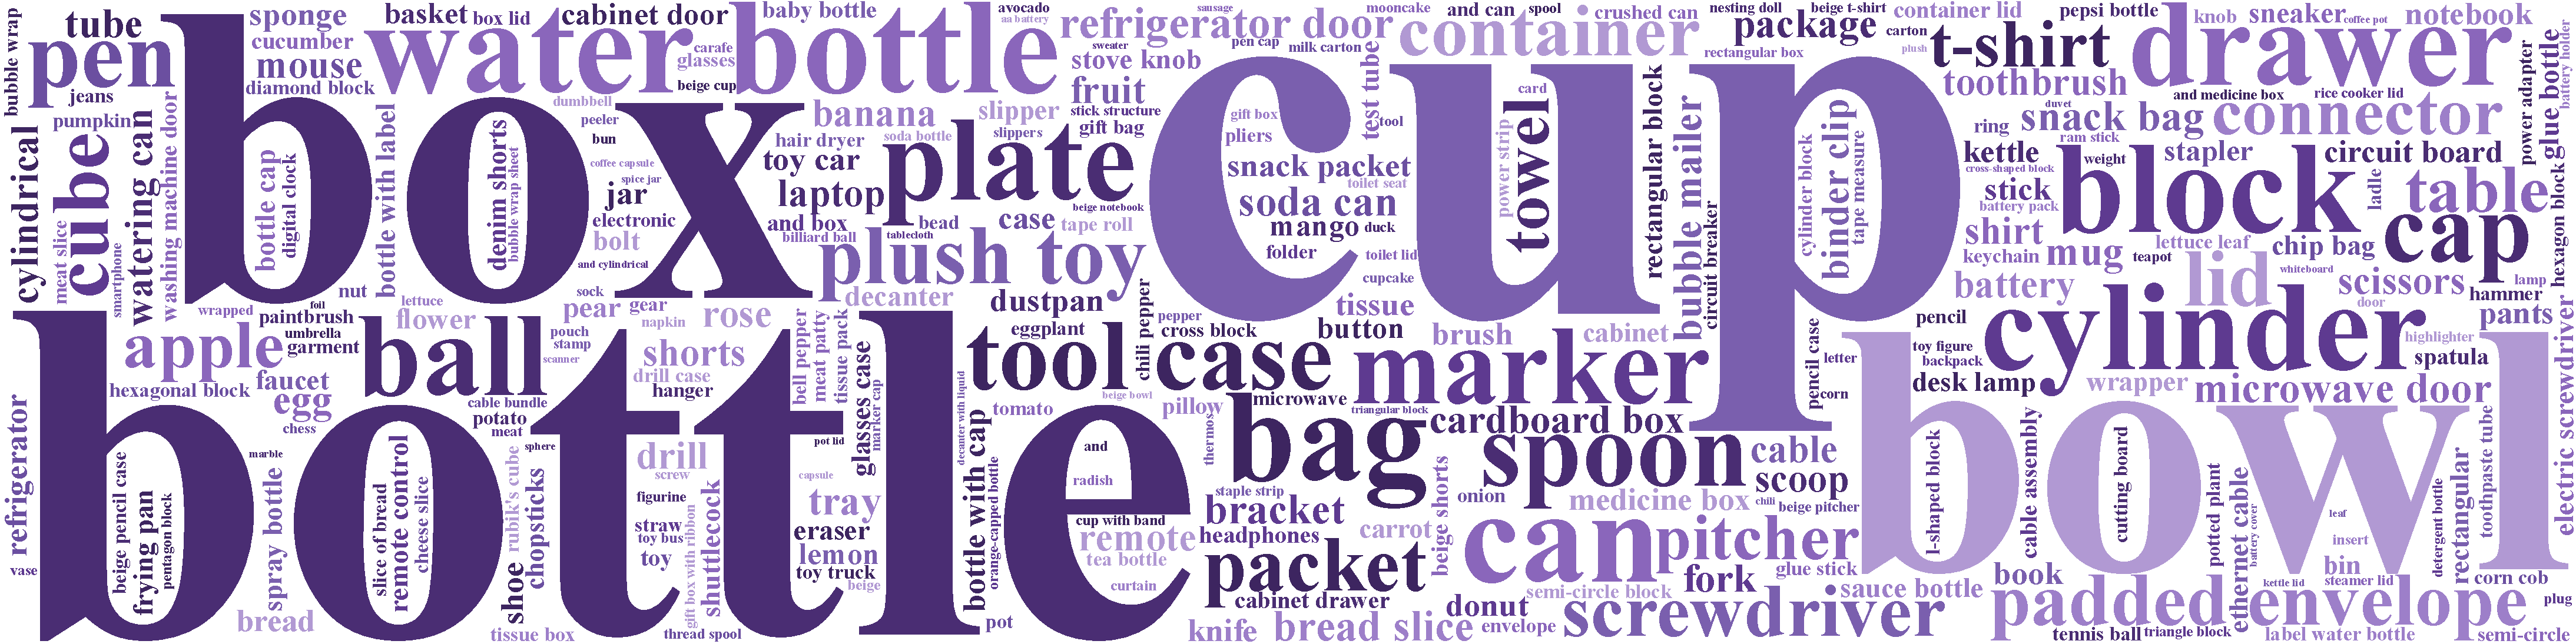
\includegraphics[width=0.8\linewidth]{figures/Data_Annotation/subtask_vocab_objects.pdf}
\caption{Word cloud of the manipulated objects in the subtask annotations, sized by frequency.}
\label{fig:object_cloud}
\end{figure}








\section{Method}


\subsection{MoE-based VLA model}
Vision-Language-Action (VLA) models pretrained on real-world cross-embodiment robot data must learn from heterogeneous trajectories characterized by misaligned action spaces, varying embodiment dynamics, and task distributions. Although the Mixture-of-Experts (MoE) mechanism provides a natural way to scale model capacity, the underlying reasons for its effectiveness in VLA pretraining remain poorly understood. In this report, we introduce a token-level loss-free MoE architecture for large-scale multi-embodiment VLA pretraining. By decoupling expert load balancing from the primary action-learning objective, and employing sigmoid-based routing confidence to allow each token to independently activate multiple experts, our design enables sparse experts to capture general representations and control logic shared across embodiments.

\noindent\textbf{Sparse MoE Architecture.}
\label{sec:moe_based_vla_model}
To facilitate convergence during cross-embodiment pretraining, we instantiate sparse MoE layers inside the action expert, which replace the feed-forward network (FFN) in the action expert. In our default configuration, all action-expert transformer blocks are equipped with MoE FFNs. Furthermore, we adopt fine-grained expert segmentation and shared expert isolation, in which a lightweight shared expert preserves universal priors, while a set of routed experts provides specialized modeling capacity.

Given the modulated FFN input $u_{\ell,t} \in \mathbb{R}^{d}$ of token $t$ at layer $\ell$, the MoE layer computes
\begin{equation}
m_{\ell}(u_{\ell,t}) =
E_{\ell}^{(s)}(u_{\ell,t})
+
\lambda
\sum_{j \in \mathcal{R}(u_{\ell,t})}
g_{\ell,j}(u_{\ell,t}) E_{\ell,j}^{(r)}(u_{\ell,t}),
\end{equation}
where $E_{\ell}^{(s)}(\cdot)$ denotes the shared expert, $E_{\ell,j}^{(r)}(\cdot)$ denotes the $j$-th routed expert, $\mathcal{R}(u_{\ell,t})$ is the selected top-$K$ routed expert set, and $\lambda$ is a routed-output scaling factor. Each shared or routed expert is implemented as a SwiGLU MLP:
\begin{equation}
E(u) = W_{\mathrm{down}}
\left(
\mathrm{SiLU}(W_{\mathrm{gate}}u) \odot W_{\mathrm{up}}u
\right).
\end{equation}
Compared with the dense FFN counterpart, both the shared and routed experts employ a smaller intermediate width, encouraging shared experts to capture general principles and routed experts to provide stronger specialization. In practice, we use one shared expert and $N_r$ routed experts per MoE layer; only $K$ routed experts are activated for each token.
For token-choice routing, we compute router logits with a linear router in FP32:
\begin{equation}
z_{\ell,j}(u_{\ell,t}) = u_{\ell,t}^{\top} e_{\ell,j},
\end{equation}
where $e_{\ell,j}$ is the learnable router embedding of the $j$-th routed expert. To avoid the strong competition among experts induced by softmax normalization, we apply a sigmoid-activated function to the router logits following DeepSeek-V3~\cite{liu2024deepseek}, the token-to-expert affinity is defined as
\begin{equation}
s_{\ell,j}(u_{\ell,t}) = \operatorname{Sigmoid}(z_{\ell,j}(u_{\ell,t})).
\end{equation}

To preserve the primary objective of action control learning in VLA models, we adopt an auxiliary-loss-free strategy inspired by DeepSeek-V3~\cite{liu2024deepseek} to promote load balancing within the MoE architecture.
Under auxiliary-loss-free balancing, each expert maintains a routing correction bias $b_{\ell,j}$. The actual mixture weights are still computed from the original unbiased affinities:
\begin{equation}
g_{\ell,j}(u_{\ell,t}) =
\frac{s_{\ell,j}(u_{\ell,t})}
{\sum_{k \in \mathcal{R}(u_{\ell,t})} s_{\ell,k}(u_{\ell,t})},
\quad j \in \mathcal{R}(u_{\ell,t}),
\end{equation}
while the selected routed expert set is determined by biased affinities:
\begin{equation}
\mathcal{R}(u_{\ell,t}) =
\mathrm{TopK}_{j}
\left(
s_{\ell,j}(u_{\ell,t}) + b_{\ell,j}, K
\right).
\end{equation}
This bias-based balancing mechanism decouples expert assignment from expert routing. Specifically, the correction bias is employed to promote load balancing, while the routing confidence remains weighted by the model's original, unbiased affinity scores.
During training, we accumulate the number of tokens assigned to each expert across micro-batches and distributed ranks. At each load-balancing update, the correction bias is adjusted according to the sign of the deviation from the mean expert load:
\begin{equation}
b_{\ell,j} \leftarrow
b_{\ell,j}
-
\gamma \cdot
\mathrm{sign}
\left(
n_{\ell,j} - \frac{1}{N_r}\sum_{k=1}^{N_r} n_{\ell,k}
\right),
\end{equation}
where $n_{\ell,j}$ is the accumulated load of expert $j$ in layer $\ell$, and $\gamma$ is the bias update speed. Optionally, the bias vector is centered after each update to prevent cumulative drift. The MoE output is then injected back through the original FFN residual branch of the action expert transformer.

\noindent\textbf{Scaling Experiments.}
To validate the efficacy of the sparse architecture under an identical compute budget, we conduct a comprehensive comparison between MoE and Dense models with strictly matched active parameter counts. Experimental results shown in \cref{fig:vla_loss_dense_vs_moe} indicate that MoE consistently achieves lower training loss and validation error than its dense counterpart. 
This advantage is observed across both optimization and generalization metrics, indicating that the performance gain of MoE does not merely arise from increased total parameter count, but from a more effective allocation of model capacity through sparse activation. These results demonstrate that, under a fixed compute budget, the sparse MoE architecture achieves more efficient scaling with reduced training loss and validation error, establishing it as a more effective scaling strategy for VLA pre-training.



\begin{figure}[H]
    \centering
    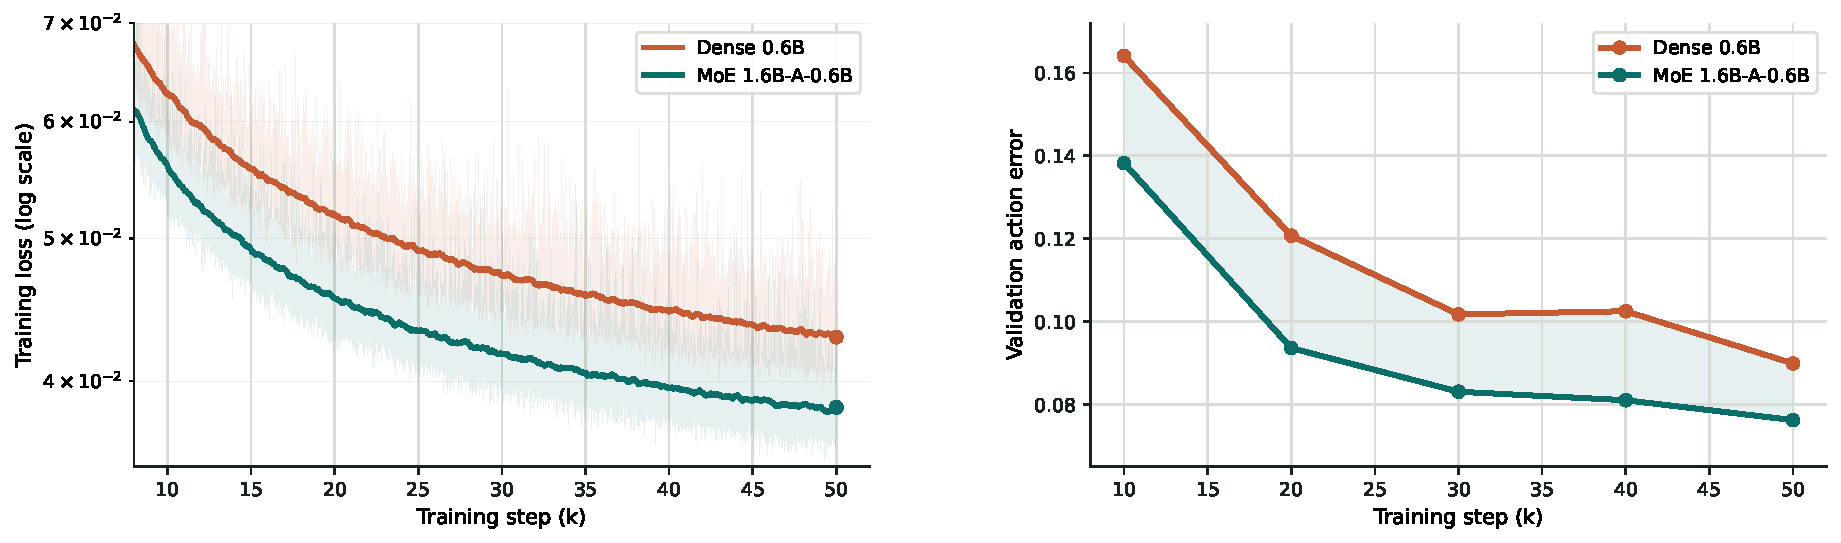
\includegraphics[width=0.96\linewidth]{figures/loss_mse_comparison.pdf}
    \caption{Comparable active-parameter scaling comparison between Dense model and MoE model using training loss on pre-training data and validation action error on GM-100 tasks.}
    \label{fig:vla_loss_dense_vs_moe}
\end{figure}

\subsection{Spatiotemporal-Aware VLA via Dual-Query Distillation}
To promote both geometric awareness and causal temporal understanding in the \method, we adopt a dual-query distillation framework inspired by recent works~\cite{wang2025vision}, where LingBot-Depth and our robotics-aware DINO-Video serve as complementary teachers.
Specifically, we append two learnable queries, $[\mathbf{Q}_t, \mathbf{Q}_{t+T}]$, to the visual and textual tokens, where $\mathbf{Q}_t$ targets the current observation and $\mathbf{Q}_{t+T}$ targets the future observation at horizon $T$ (\textit{i.e.}, the action chunk size). These contextualized query states are then distilled from two complementary teachers: a depth teacher, LingBot-Depth~\cite{lingbotdepth}, which provides explicit geometric supervision, and a causal video teacher, \dinomodel, which provides temporally grounded visual representations.

\noindent\textbf{LingBot-Depth for geometric supervision.}
To inject explicit spatial and geometric priors into \method, we align the dual-query states with depth tokens extracted from LingBot-Depth. Specifically, the current and future queries, $[\mathbf{Q}_t, \mathbf{Q}_{t+T}]$, are trained to predict the corresponding depth representations $[\mathbf{D}_t, \mathbf{D}_{t+T}]$ from the current and future manipulation frames, respectively. The depth distillation objective is
\begin{align}
\mathcal{L}_{depth}
=
\mathbb{E}\left[
\left\|\mathrm{Proj}_{depth}(\mathbf{Q}_t)-\mathbf{D}_t\right\|_1
+
\left\|\mathrm{Proj}_{depth}(\mathbf{Q}_{t+T})-\mathbf{D}_{t+T}\right\|_1
\right],
\label{eq:depth_distill}
\end{align}
where $\mathrm{Proj}_{depth}(\cdot)$ denotes a projection module with cross-attention for dimensional alignment. 
Within the causal VLM architecture, $\mathbf{Q}_t$ captures the immediate scene geometry, while $\mathbf{Q}_{t+T}$ learns to anticipate future geometric configurations relevant to upcoming manipulation.

\noindent\textbf{Causal \dinomodel for temporal supervision.}
While depth supervision provides geometric structure, it does not capture the causal temporal dynamics required for robotic control. Motivated by the success of latent visual representations across a broad range of action and robotics applications~\cite{larybench, beingH07, lda1b, dexWorldModel, lawam, wog}, we introduce \dinomodel, a robotics-aware video representation model built on top of the DINOv3~\cite{dinov3} image backbone. Unlike image-level features extracted independently for each frame, \dinomodel produces motion-aware visual representations with causal temporal attention, such that the feature at each time step depends only on the current and past observations.
Given the contextualized query states $[\mathbf{Q}_t, \mathbf{Q}_{t+T}]$, the current query is trained to predict the \dinomodel feature of the current frame, while the future query is trained to predict the feature of the future frame at horizon $T$. Denoting the teacher targets by $[\mathbf{Z}_t, \mathbf{Z}_{t+T}]$, extracted from a single causal forward pass of \dinomodel over the corresponding observation clip, the video distillation objective is
\begin{align}
\mathcal{L}_{video}
=
\mathbb{E}\left[
\left\|\mathrm{Proj}_{video}(\mathbf{Q}_t)-\mathbf{Z}_t\right\|_F^2
+
\left\|\mathrm{Proj}_{video}(\mathbf{Q}_{t+T})-\mathbf{Z}_{t+T}\right\|_F^2
\right],
\label{eq:dino_video}
\end{align}
where $\mathrm{Proj}_{video}(\cdot)$ maps the query states into the patch-level feature space of \dinomodel. This objective encourages \method to recover both the current motion-aware representation and its future counterpart, complementing the geometric supervision from depth distillation.

\noindent\textbf{Details of robotics-aware \dinomodel.}
We initialize \dinomodel from DINOv3 and extend it with block-wise causal temporal attention and 3D rotary positional embeddings (3D-RoPE)~\cite{videorope}, enabling causal video modeling while preserving the spatial semantics and geometry priors inherited from DINOv3. 
We train \dinomodel on 5M video clips spanning Internet, egocentric, and robotic data, using video-adapted DINO and iBOT self-distillation objectives~\cite{omnistream}. 
For each sample, we uniformly sample 16 frames and assign an absolute temporal encoding based on the effective frame rate to distinguish clips with different real-time spans~\cite{cosmos3}. 
On LARYBench~\cite{larybench}~(see \cref{tab:larybench}), \dinomodel achieves the best performance on three of four benchmarks, supporting its effectiveness as a robotics-aware temporal teacher.





\begin{table*}[h]
\centering
\caption{Results of \dinomodel on LARYBench Classification and Regression Evaluation.}
\label{tab:larybench}
\begin{tabular}{llcccc}
\toprule
\multirow{2}{*}{Model} & \multirow{2}{*}{Params(M)} & \multicolumn{2}{c}{Classification}  & \multicolumn{2}{c}{Regression} \\
 & & \textit{Composite Human}$\uparrow$ & \textit{Composite Robot}$\uparrow$ & \textit{RoboCOIN}$\downarrow$ & \textit{AgiBotWorld-Beta}$\downarrow$ \\
\midrule
V-JEPA 2~\cite{vjepa2} & 303.89 &\textbf{ 80.35} & 70.43 & 0.32 & 0.33 \\
DINOv3~\cite{dinov3} & 303.13 & 76.19 & 69.06 & 0.22 & 0.24\\

\midrule
\dinomodel & 303.13 & {80.21} & \textbf{71.97} & \textbf{0.20} & \textbf{0.19}\\
\bottomrule

\end{tabular}
\end{table*}
